\clearpage
\part{Matched confirmation and prospective audit}
\section{Recipe effects under matched training}\label{sec:matched-confirmation}\label{sec:matched-followup}
The follow-up tests two weaknesses in the earlier evidence: the absence of freshly fitted C0 anchors under the final training engine, and the limited independent RGB assessment. Its protocol fixes the comparisons before the new runs. The grayscale and RGB experiments remain separate tasks; the RGB cohort does not provide a new test for Fashion-MNIST.

For each Fashion-MNIST family, the original C0 recipe and the frozen OPT3-selected recipe are trained for 60 epochs with fresh seeds 1009, 2027 and 3037. Paired arms share the exact 54,000/6,000 split, engine, architecture dimensions, initialization policy and loader seed. Recipe order alternates by seed. Each trajectory supplies minimum-CE, maximum-F1 and fixed-epoch-60 checkpoints: 30 fits yield 90 checkpoint cells, not 90 independent fits.

The prespecified primary contrast is selected recipe minus C0 for the CNN at epoch 60. Other families, adaptive checkpoint policies and their interaction are secondary descriptive comparisons. The design separates a recipe bundle from checkpoint selection, rather than isolating individual learning-rate, regularization or scheduling effects.

\begin{center}\small
\setlength{\tabcolsep}{4pt}
\begin{tabular}{lrrrr}\toprule
Family & C0, epoch 60 & Selected, epoch 60 & Paired difference & Positive pairs\\\midrule
Linear & $0.86280\pm0.00211$ & $0.86618\pm0.00094$ & $+0.00338\pm0.00143$ & 3/3\\
MLP & $0.90218\pm0.00236$ & $0.91109\pm0.00206$ & $+0.00891\pm0.00115$ & 3/3\\
CNN & $0.92823\pm0.00087$ & $0.92914\pm0.00273$ & $+0.00091\pm0.00351$ & 1/3\\
GRU & $0.90293\pm0.00298$ & $0.90615\pm0.00278$ & $+0.00322\pm0.00374$ & 2/3\\
Transformer & $0.90228\pm0.00297$ & $0.91174\pm0.00087$ & $+0.00946\pm0.00247$ & 3/3\\\bottomrule
\end{tabular}\end{center}
All scores are Macro-F1, with mean $\pm$ sample SD over three seeds. Difference SD is calculated from paired seed differences. These are descriptive SDs on a fixed, previously inspected validation split, not population confidence intervals.

\subsection{The primary CNN gain is small and inconsistent}
The primary mean difference is $+0.000912$ F1, or $0.0912$ F1 percentage points. Its paired differences are $+0.004894$, $-0.001738$ and $-0.000419$ for seeds 1009, 2027 and 3037. Only one pair favors C5, and the paired SD of 0.003511 exceeds the mean effect. This does not establish a stable recipe improvement. C5 also has greater between-seed variability at epoch 60 than C0 in this run.

MLP and Transformer have larger positive final-epoch differences in all three pairs. These secondary outcomes support better late-trajectory behavior for their selected recipes under the declared protocol. They remain conditional on configurations chosen during earlier development and on a reused validation sample. Fresh training seeds reduce dependence on one initialization; they do not create fresh evaluation images.

\clearpage
\section{Checkpoint dependence and objective trade-offs}
\begin{center}\small
\setlength{\tabcolsep}{5pt}
\begin{tabular}{lrrrrrr}\toprule
& \multicolumn{2}{c}{Minimum CE} & \multicolumn{2}{c}{Maximum F1} & \multicolumn{2}{c}{Epoch 60}\\
Family & C0 & Selected & C0 & Selected & C0 & Selected\\\midrule
Linear & 0.86504 & 0.86481 & 0.86830 & 0.86806 & 0.86280 & 0.86618\\
MLP & 0.90200 & 0.91021 & 0.90866 & 0.91360 & 0.90218 & 0.91109\\
CNN & 0.92877 & 0.92940 & 0.92991 & 0.93126 & 0.92823 & 0.92914\\
GRU & 0.90962 & 0.90959 & 0.91294 & 0.91278 & 0.90293 & 0.90615\\
Transformer & 0.90630 & 0.90592 & 0.91022 & 0.91326 & 0.90228 & 0.91174\\\bottomrule
\end{tabular}\end{center}
Entries are mean validation Macro-F1 over the same three seeds. All checkpoints in a row/arm derive from its shared 60-epoch trajectories.

The CNN recipe difference is $+0.000635$ at the CE-selected checkpoint and $+0.001351$ at the F1-selected checkpoint. The latter favors C5 in all three pairs, but it is a secondary adaptive comparison and does not override the weak primary result. The recipe-by-selector interaction,
\[
  (\mathrm{selected}_{F1}-\mathrm{C0}_{F1})
  -(\mathrm{selected}_{CE}-\mathrm{C0}_{CE}),
\]
is $+0.000716\pm0.001736$ for the CNN. Its variation across three pairs does not support a population interaction claim.

For Linear, cosine scheduling improves epoch-60 F1 by 0.00338 while recipe differences at CE/F1-selected checkpoints are approximately zero ($-0.00023/-0.00024$). GRU shows the same pattern: $+0.00322$ at epoch 60, but $-0.00003/-0.00016$ after CE/F1 selection. Transformer has differences $+0.00946$, $-0.00038$ and $+0.00304$ at final, CE and F1 checkpoints respectively. Thus an improvement at the end of training is not interchangeable with superiority of a validation-selected checkpoint.

\subsection{Higher selected validation F1 does not establish generalization}
Maximum-F1 selection explicitly maximizes the same validation score reported here. Its score being at least as high as that of the CE-selected checkpoint on those images is expected by construction. The within-trajectory comparison describes the choice of objective; it cannot independently demonstrate better generalization.

The losses illustrate the distinction. For MLP C0, mean validation CE is 0.27457 at the CE checkpoint, 0.32177 at the F1 checkpoint and 0.40553 at epoch 60. A checkpoint with higher F1 can have worse probability loss. The final-epoch primary endpoint avoids within-trajectory validation selection, but it still uses images repeatedly inspected during project development. No official-test evaluation is performed in this follow-up.

\subsection{Completion and numerical portability}
All 30 trajectories finish 60 epochs and 25,320 optimizer updates. The A100 controller records 15,335.76 active seconds (4.260 hours), excluding setup and the initial software smoke test. The environment is PyTorch 2.11.0+cu130, torchvision 0.26.0+cu130, NumPy 2.4.2, scikit-learn 1.8.0 and Python 3.13 on an NVIDIA A100-SXM4-40GB.

Independent reconstruction verifies all 540,000 prediction rows, 90 cells, 1,800 history rows, validation IDs and checkpoint epochs (maximum metric difference $2.23\times10^{-16}$). NLL checks aggregate the saved per-image values. Read-only CPU/PyTorch 2.10 replay strictly loads all 90 checkpoints, recording 11 label differences across 540,000 cell-image predictions and maximum cell mean-NLL difference $1.55\times10^{-5}$. Tables retain the original A100 values; exact cross-runtime identity is not claimed. The primary CNN conclusion is unchanged.

\clearpage
\section{A prospectively fixed RGB cohort}\label{sec:prospective-rgb}\label{sec:prospective-followup}
\subsection{Cohort construction and fixed model identities}
The new audit uses photographs from Fashionpedia training license IDs 3/5, excluded by the earlier 0/1/6 filter. Six previously fitted C0/C4 checkpoints, seeds 314/2718/5772, preprocessing, the C4 seed-314 review policy and analysis are frozen before cohort preparation. There is no new RGB fitting, calibration or threshold selection.

Source-URL groups are ranked by SHA256 with seed 20261029. The first 2,000 groups are committed before target-category filtering, without replacement after exclusions. Recorded image IDs, source URLs, previews and quarantines are excluded. Transitive exact-pixel/perceptual-hash components touching historical images are removed. These controls reduce detectable overlap but cannot guarantee separation of every person, outfit or undetected near-duplicate.

The final cohort contains 2,766 annotated crops in 1,826 source/duplicate components. Inference was completed locally on CPU before the Colab confirmation run. Colab reuses the frozen audit evidence byte for byte; this is not a second independent RGB evaluation. The cohort remains a project-unused, same-source license-shift audit, rather than an external or IID benchmark. Unrecorded prior viewing and pretrained-model exposure cannot be excluded. Photographs and prepared crops are not redistributed.

\begin{center}\small
\begin{tabular}{lrrrr}\toprule
Category & Crops & Components & C0 mean F1 & C4 mean F1\\\midrule
Shirt/blouse & 182 & 175 & 0.5633 & 0.5659\\
Top/T-shirt/sweatshirt & 856 & 811 & 0.8123 & 0.8208\\
Jacket & 300 & 279 & 0.7211 & 0.7395\\
Pants & 476 & 461 & 0.9091 & 0.9185\\
Skirt & 257 & 253 & 0.7840 & 0.7856\\
Dress & 695 & 684 & 0.8572 & 0.8589\\\bottomrule
\end{tabular}\end{center}
Components can contain several categories, so class-level component counts do not sum to the cohort total. Shirt/blouse remains the weakest category despite greater support than the original assessment; aggregate accuracy does not describe uniform class performance.

\subsection{A favorable point estimate with unresolved uncertainty}
\begin{center}\small
\setlength{\tabcolsep}{4pt}
\begin{tabular}{lrrrr}\toprule
Cohort & C0 F1 & C4 F1 & Difference & Paired 95\% interval\\\midrule
Earlier assessment (327) & 0.77472 & 0.76638 & $-0.00834$ & $[-0.03820,+0.01829]$\\
Project-unused cohort (2,766) & 0.77449 & 0.78154 & $+0.00705$ & $[-0.00036,+0.01512]$\\\bottomrule
\end{tabular}\end{center}
The prespecified RGB endpoint is C4 minus C0 mean Macro-F1 over three paired fixed models. On the new cohort the mean difference is $+0.007046$, or 0.7046 F1 percentage points. A 2,000-replicate paired percentile bootstrap resamples the 1,826 source/duplicate components jointly, with seed 20261030. Its interval includes zero. It describes component-sampling uncertainty conditional on these six models, without seed-population, external-data or deployment guarantees. It establishes neither a positive effect nor equivalence. The opposite direction on the earlier assessment is retained.

\clearpage
\section{Frozen review policy by garment class}\label{sec:policy-by-class}
\subsection{Global result and true-class behavior}
This diagnostic concerns the single, preselected C4 seed-314 model. It is separate from the preceding three-seed mean-F1 comparison. For logits $z_i$, the policy computes $\pi_i=\operatorname{softmax}(z_i/T)$ with the frozen temperature $T=5.345757234366385$, predicts $\hat Y_i=\arg\max_k\pi_{ik}$, and accepts when
\[
 A_i=\mathbf{1}\!\left[\max_k\pi_{ik}\geq0.88\right].
\]
The remaining crops are referred for review. Positive temperature scaling leaves the predicted class unchanged. No weights, temperature or threshold are fitted or changed in this post-hoc analysis of stored logits and labels.

The policy accepts 1,506/2,766 crops (54.45\% coverage), of which 1,445 are correct (95.95\% accepted accuracy). It refers 1,260 crops and retains 61 errors among accepted predictions. Full-cohort accuracy remains 82.1041\% and Macro-F1 0.783914. These different denominators describe different aspects of the same fixed model.

For a true class $Y=c$, coverage measures its accepted fraction, and accepted accuracy measures correctness within that fraction:
\[
 \widehat C^Y_c=\frac{\sum_i A_i\mathbf{1}(Y_i=c)}{\sum_i\mathbf{1}(Y_i=c)},
 \qquad
 \widehat a^{Y,A}_c=\frac{\sum_i A_i\mathbf{1}(Y_i=\hat Y_i=c)}{\sum_i A_i\mathbf{1}(Y_i=c)}.
\]
\begin{center}\small
\setlength{\tabcolsep}{4pt}
\begin{tabular}{lrrrrr}\toprule
True category & Accepted/total & Correct/accepted & Review & \shortstack{Coverage\\(\%)} & \shortstack{Accepted\\accuracy (\%)}\\\midrule
Shirt/blouse & 33/182 & 22/33 & 149 & 18.13 & 66.67\\
\shortstack[l]{Top/T-shirt/\\sweatshirt} & 431/856 & 406/431 & 425 & 50.35 & 94.20\\
Jacket & 82/300 & 76/82 & 218 & 27.33 & 92.68\\
Pants & 361/476 & 360/361 & 115 & 75.84 & 99.72\\
Skirt & 106/257 & 100/106 & 151 & 41.25 & 94.34\\
Dress & 493/695 & 481/493 & 202 & 70.94 & 97.57\\\midrule
Total & 1,506/2,766 & 1,445/1,506 & 1,260 & 54.45 & 95.95\\\bottomrule
\end{tabular}\end{center}
The global result masks substantial class variation. Of 182 true shirt/blouse crops, 149 are referred; 11 of the 33 accepted crops are still misclassified. Pants have much higher coverage and only one error among 361 accepted crops. Shirt/blouse contributes 2.19\% of the accepted set but 18.03\% of its errors. A high pooled accepted accuracy therefore does not establish reliable handling of every garment category.

This grouping evaluates labeled audit data. The true class is unavailable when a new crop arrives, so these rows cannot directly specify an online class-dependent acceptance rule. The small accepted shirt/blouse count also limits precision of its rate estimate. The counts are descriptive outcomes on this cohort, not per-class accuracy guarantees.

\clearpage
\subsection{Predicted outputs and review workload}
Grouping by predicted class answers a different question: how reliable is an accepted output labeled $c$? Predicted-class coverage estimates $\Pr(A=1\mid\hat Y=c)$, while accepted precision estimates $\Pr(Y=c\mid A=1,\hat Y=c)$. The denominators now include all predictions of $c$, rather than all crops whose true class is $c$. Predicted labels are observable online; measuring their precision still requires ground-truth audit labels.

\begin{center}\small
\setlength{\tabcolsep}{4pt}
\begin{tabular}{lrrrrr}\toprule
Predicted output & \shortstack{Accepted/\\predictions} & Correct/accepted & Review & \shortstack{Coverage\\(\%)} & \shortstack{Accepted\\precision (\%)}\\\midrule
Shirt/blouse & 24/183 & 22/24 & 159 & 13.11 & 91.67\\
\shortstack[l]{Top/T-shirt/\\sweatshirt} & 428/856 & 406/428 & 428 & 50.00 & 94.86\\
Jacket & 88/284 & 76/88 & 196 & 30.99 & 86.36\\
Pants & 362/484 & 360/362 & 122 & 74.79 & 99.45\\
Skirt & 101/243 & 100/101 & 142 & 41.56 & 99.01\\
Dress & 503/716 & 481/503 & 213 & 70.25 & 95.63\\\midrule
Total & 1,506/2,766 & 1,445/1,506 & 1,260 & 54.45 & 95.95\\\bottomrule
\end{tabular}\end{center}
Accepted jacket outputs have the lowest observed precision, 76/88 = 86.36\%. Accepted outputs labeled shirt/blouse have precision 22/24 = 91.67\%; this is not the 22/33 true-class accepted accuracy in the preceding table. The two rates condition on different events and must not be interchanged.

The accepted confusion counts explain why this distinction matters. The 11 accepted errors on true shirt/blouse crops are labeled jacket (five), top/T-shirt/sweatshirt (four) or dress (two). A change applied only to outputs predicted as shirt/blouse would not directly address those 11 cases. Of the 12 false accepted jacket outputs, six are true tops, five are true shirts/blouses and one is a true dress. These are observed confusion patterns, without a claim about their visual cause.

Across all classes, the model makes 495 full-cohort errors. The policy refers 434 of them for review (87.68\%) and accepts the other 61. The review stream also contains 826 predictions that were already correct. Referral therefore trades automatic coverage for review workload; it does not measure how accurately a human would resolve those crops. Human-review outcomes, processing time and costs are unmeasured.

\subsection{Scope of the policy conclusion}
This class breakdown was added after cohort outcomes were inspected. Crops share source/duplicate components, and small accepted subsets warrant caution. The earlier representative-level calibration bound was neither a per-class certificate nor a guarantee for this license-shifted population. Neither table establishes that every class meets 95\% accepted accuracy. Conditioning on the true label also differs from conditioning on confidence, so the shirt/blouse row is not a direct test of probability calibration.

A class-aware policy would require its own suitable calibration evidence and a prespecified evaluation on another untouched cohort. No such policy is selected here, and the threshold remains 0.88. The matched recipe and grouped RGB comparisons retain their earlier conclusions. This diagnostic qualifies the interpretation of selective operation without replacing either primary endpoint or the recorded local-serving and ONNX limitations.

\clearpage
\section{Paired diagnostic plots}
\begin{figure}[H]
\centering
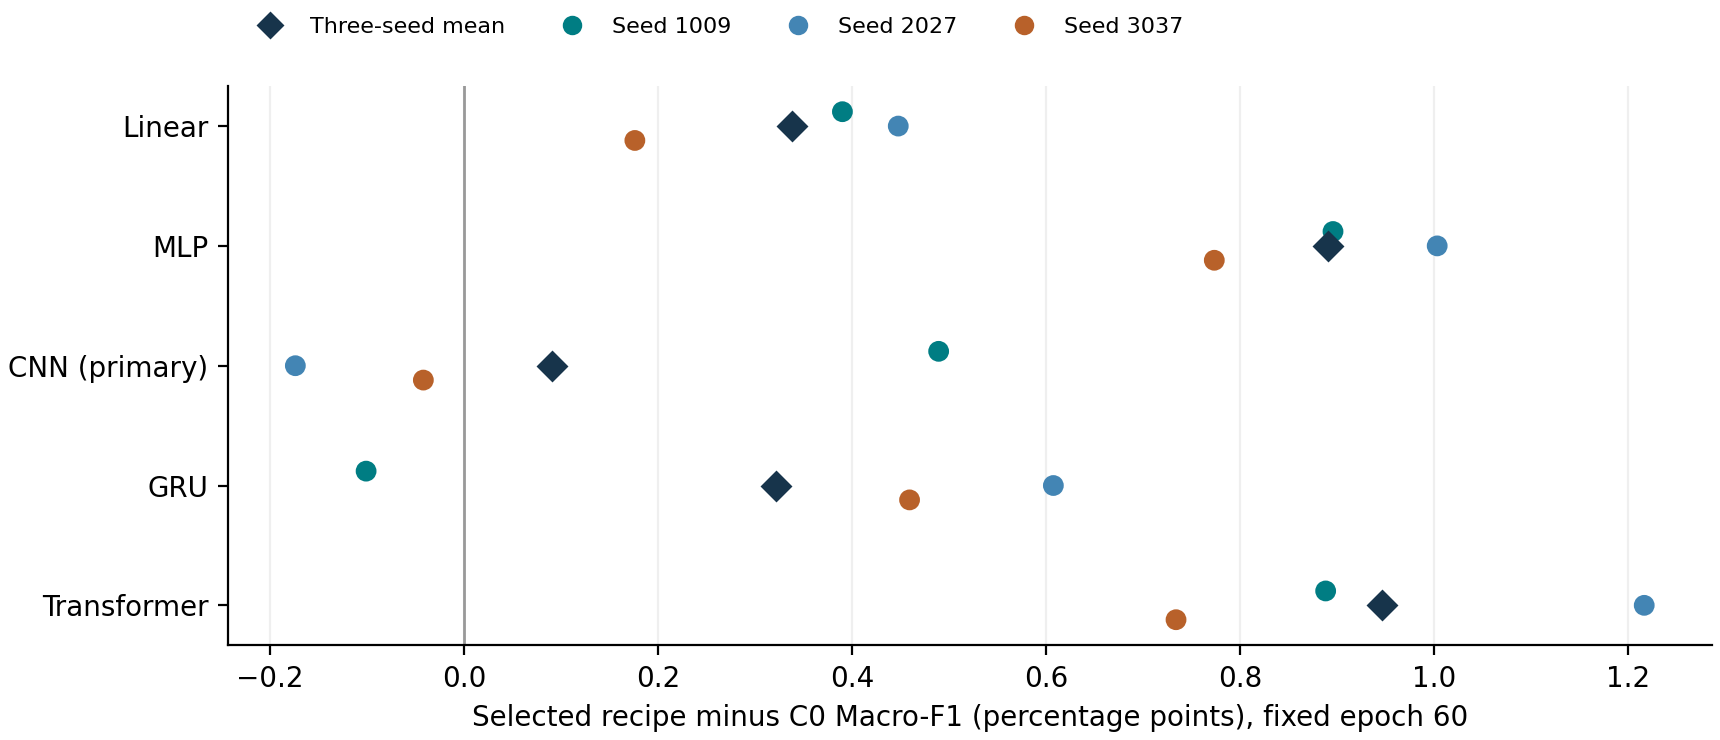
\includegraphics[width=\linewidth]{figures/matched_epoch60_deltas.png}
\caption{Fixed-epoch-60 recipe differences on the old validation partition. Each circle is one paired training seed; diamonds are three-seed means. The prespecified primary family is CNN. The displayed dispersion concerns training seeds on one fixed split, without a new image-population confidence claim.}
\end{figure}
\begin{figure}[H]
\centering
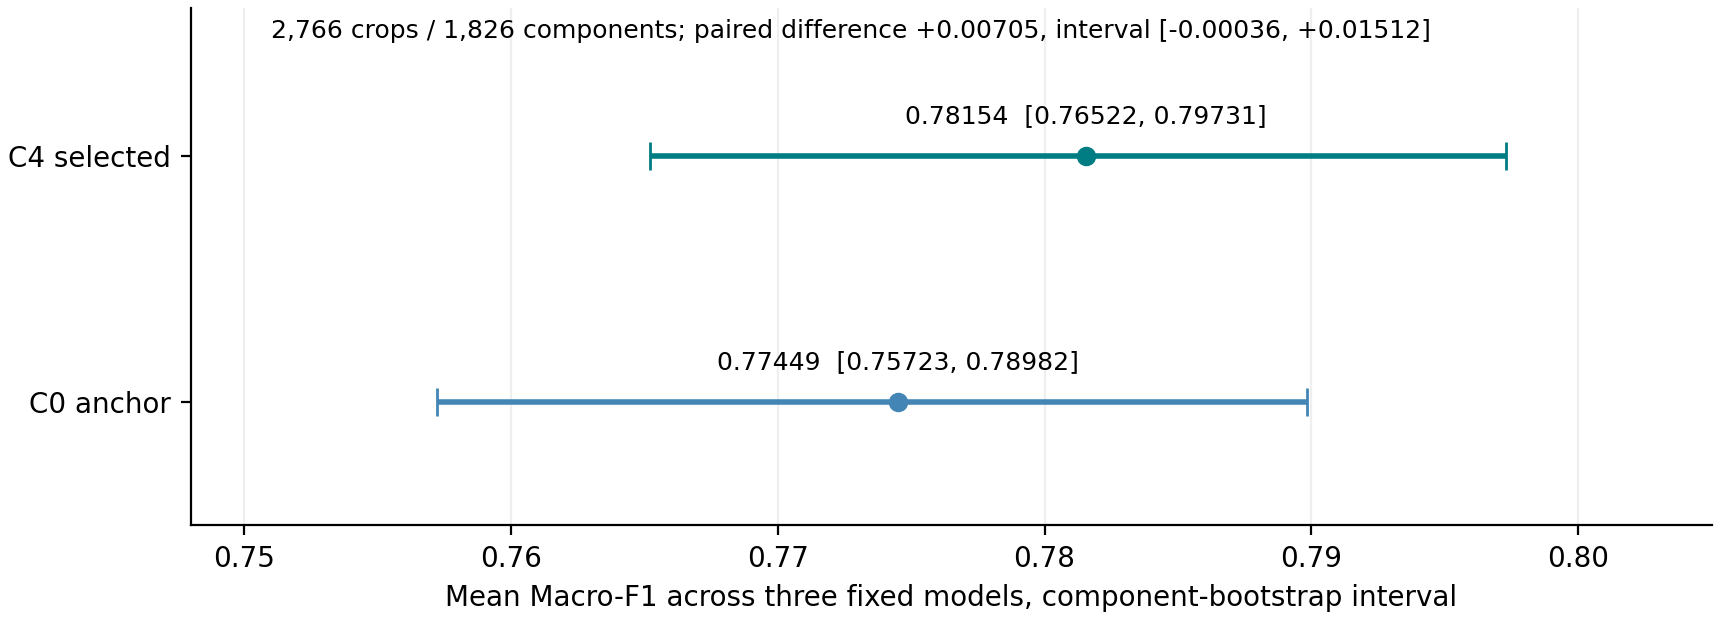
\includegraphics[width=\linewidth]{figures/prospective_rgb_intervals.png}
\caption{Mean Macro-F1 on the project-unused RGB cohort. Marginal component-bootstrap intervals describe the six fixed fitted models. The joint paired difference interval, shown in the plot, is the relevant recipe contrast and includes zero. Overlap of marginal intervals is not used as a significance test.}
\end{figure}
